\section{Appendix}

\subsection{Real robot pictures}
\label{sec:real_pictures}
\begin{figure}[H]
    \centering
    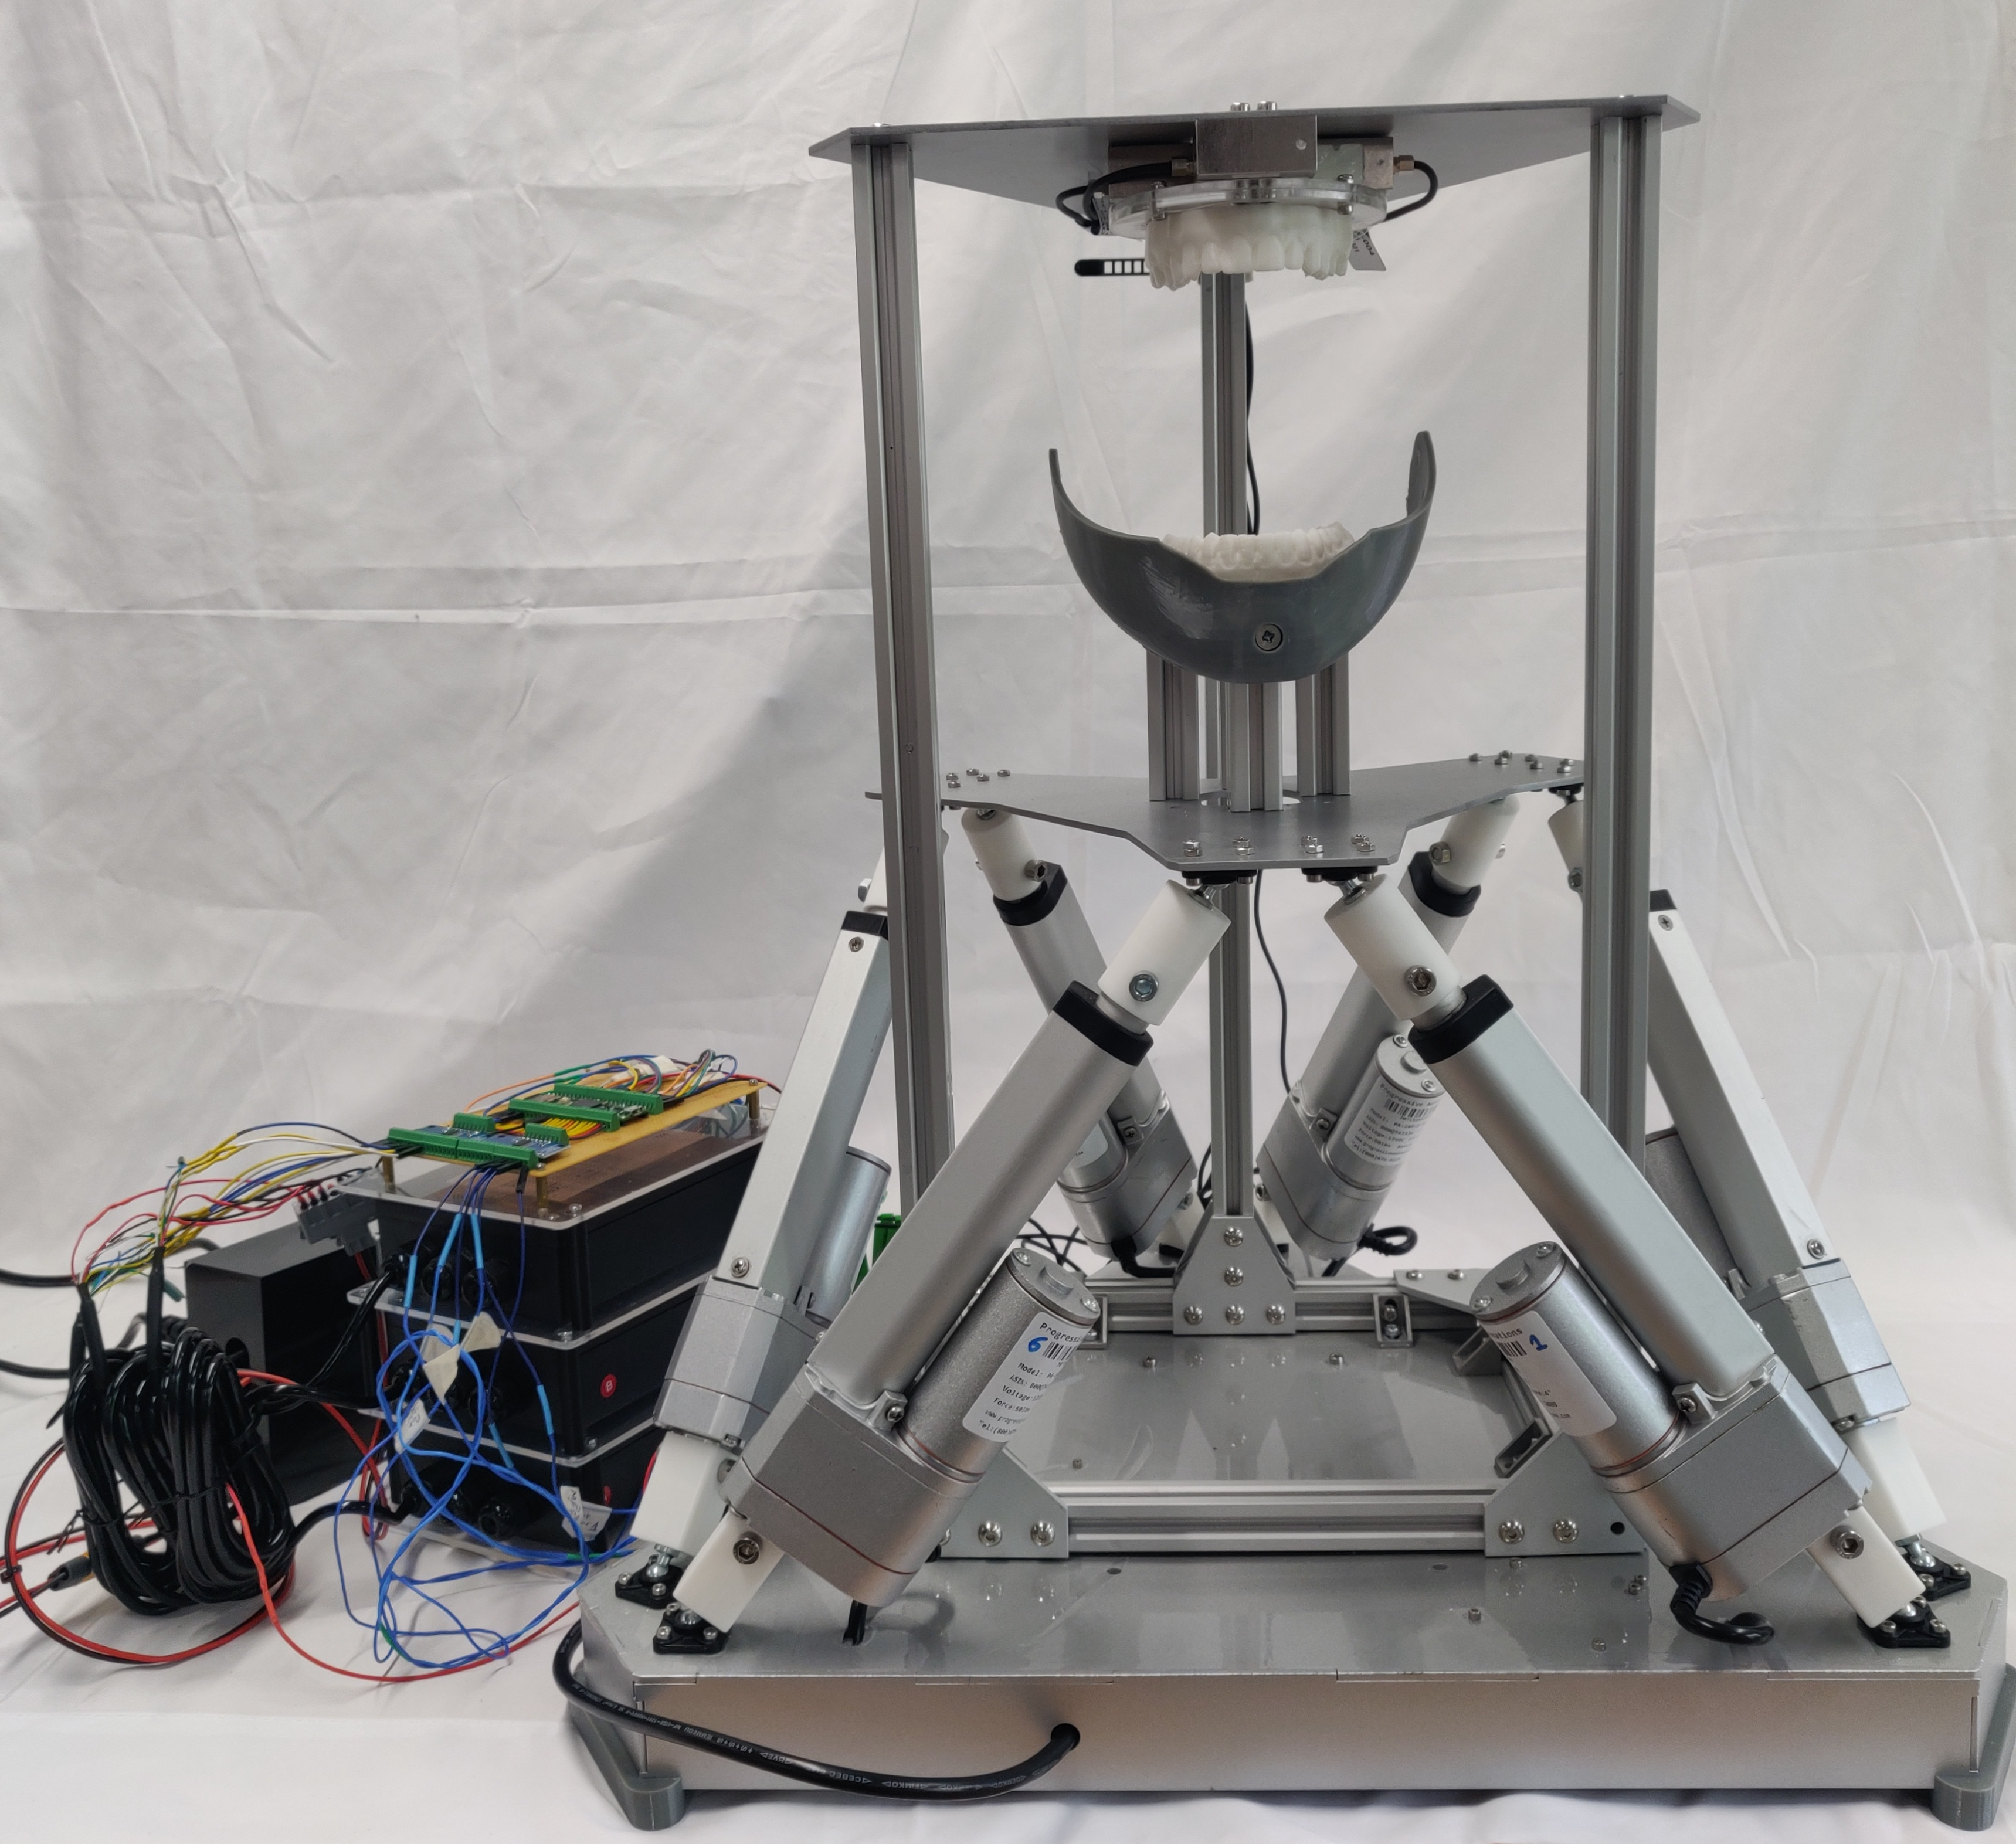
\includegraphics[width=0.8\textwidth]{figures/overview_real.jpg}
    \caption{Picture of the robot overview, including electronics on the left side.}
    \label{fig:overview_real}
\end{figure}

\begin{figure}[H]
    \centering
    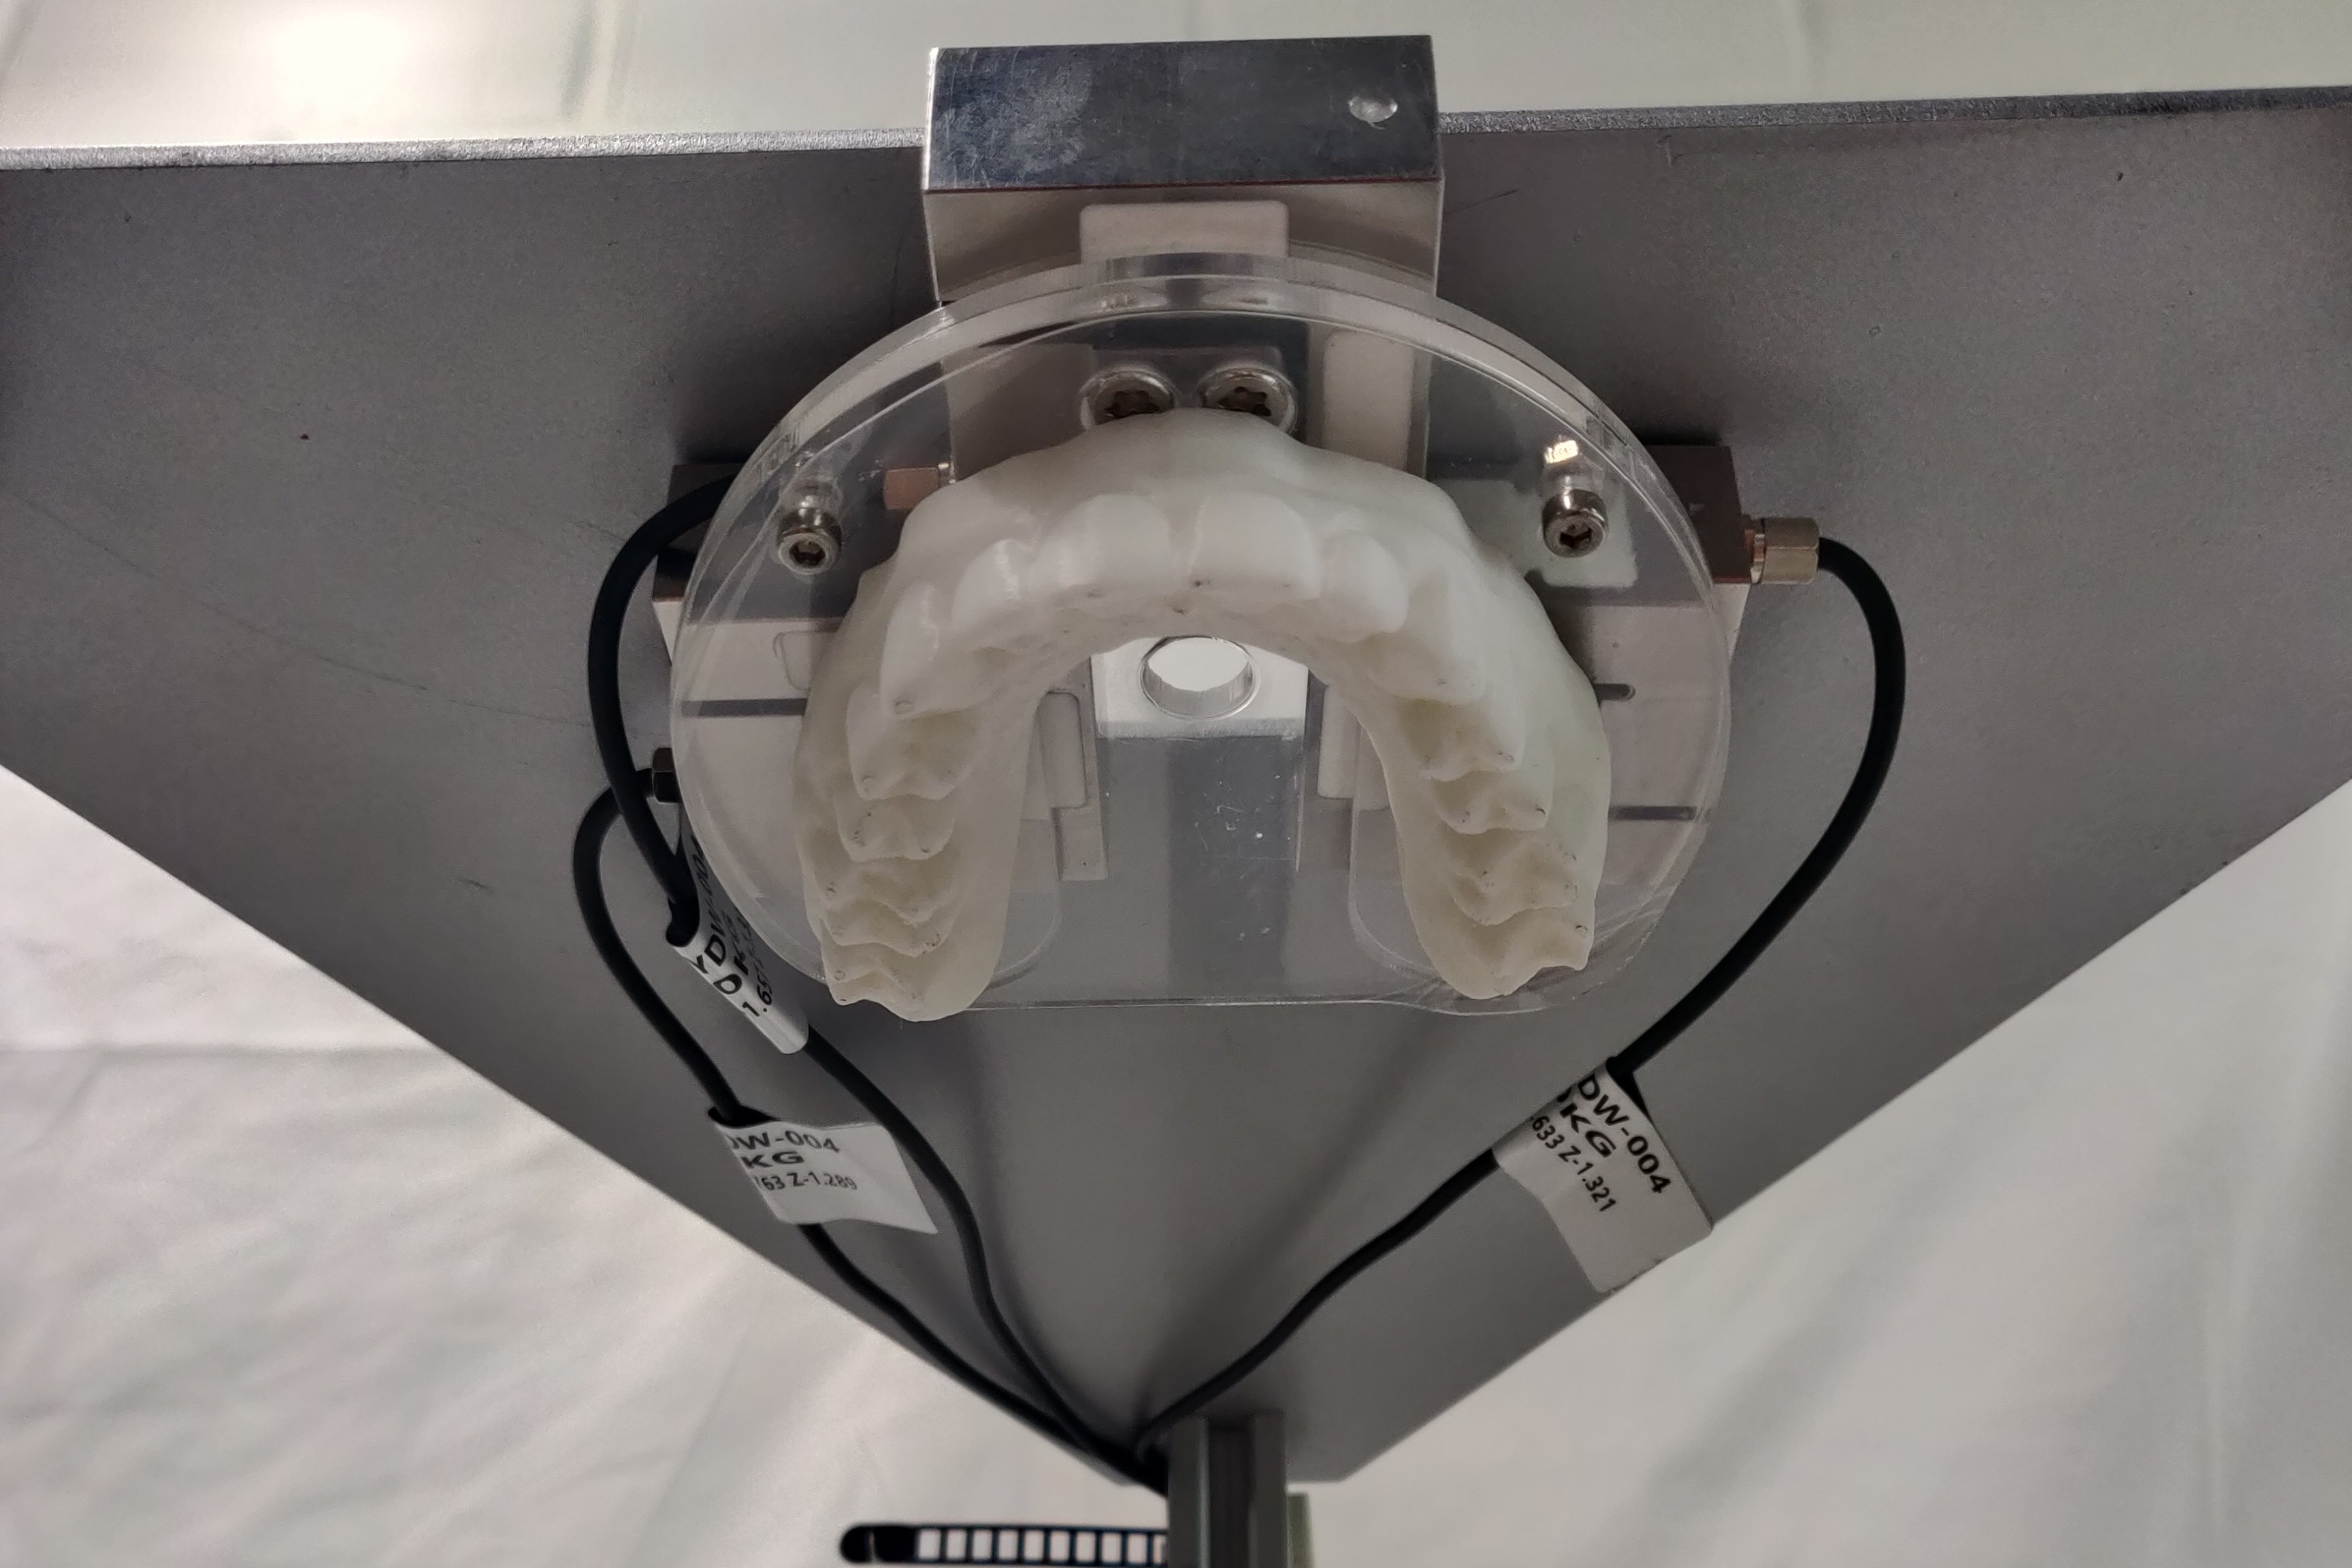
\includegraphics[width=0.6\textwidth]{figures/upper_jaw_close_up.jpg}
    \caption{Picture of the upper jaw close-up.}
    \label{fig:pic_upper_jaw_close_up}
\end{figure}

\begin{figure}[H]
    \centering
    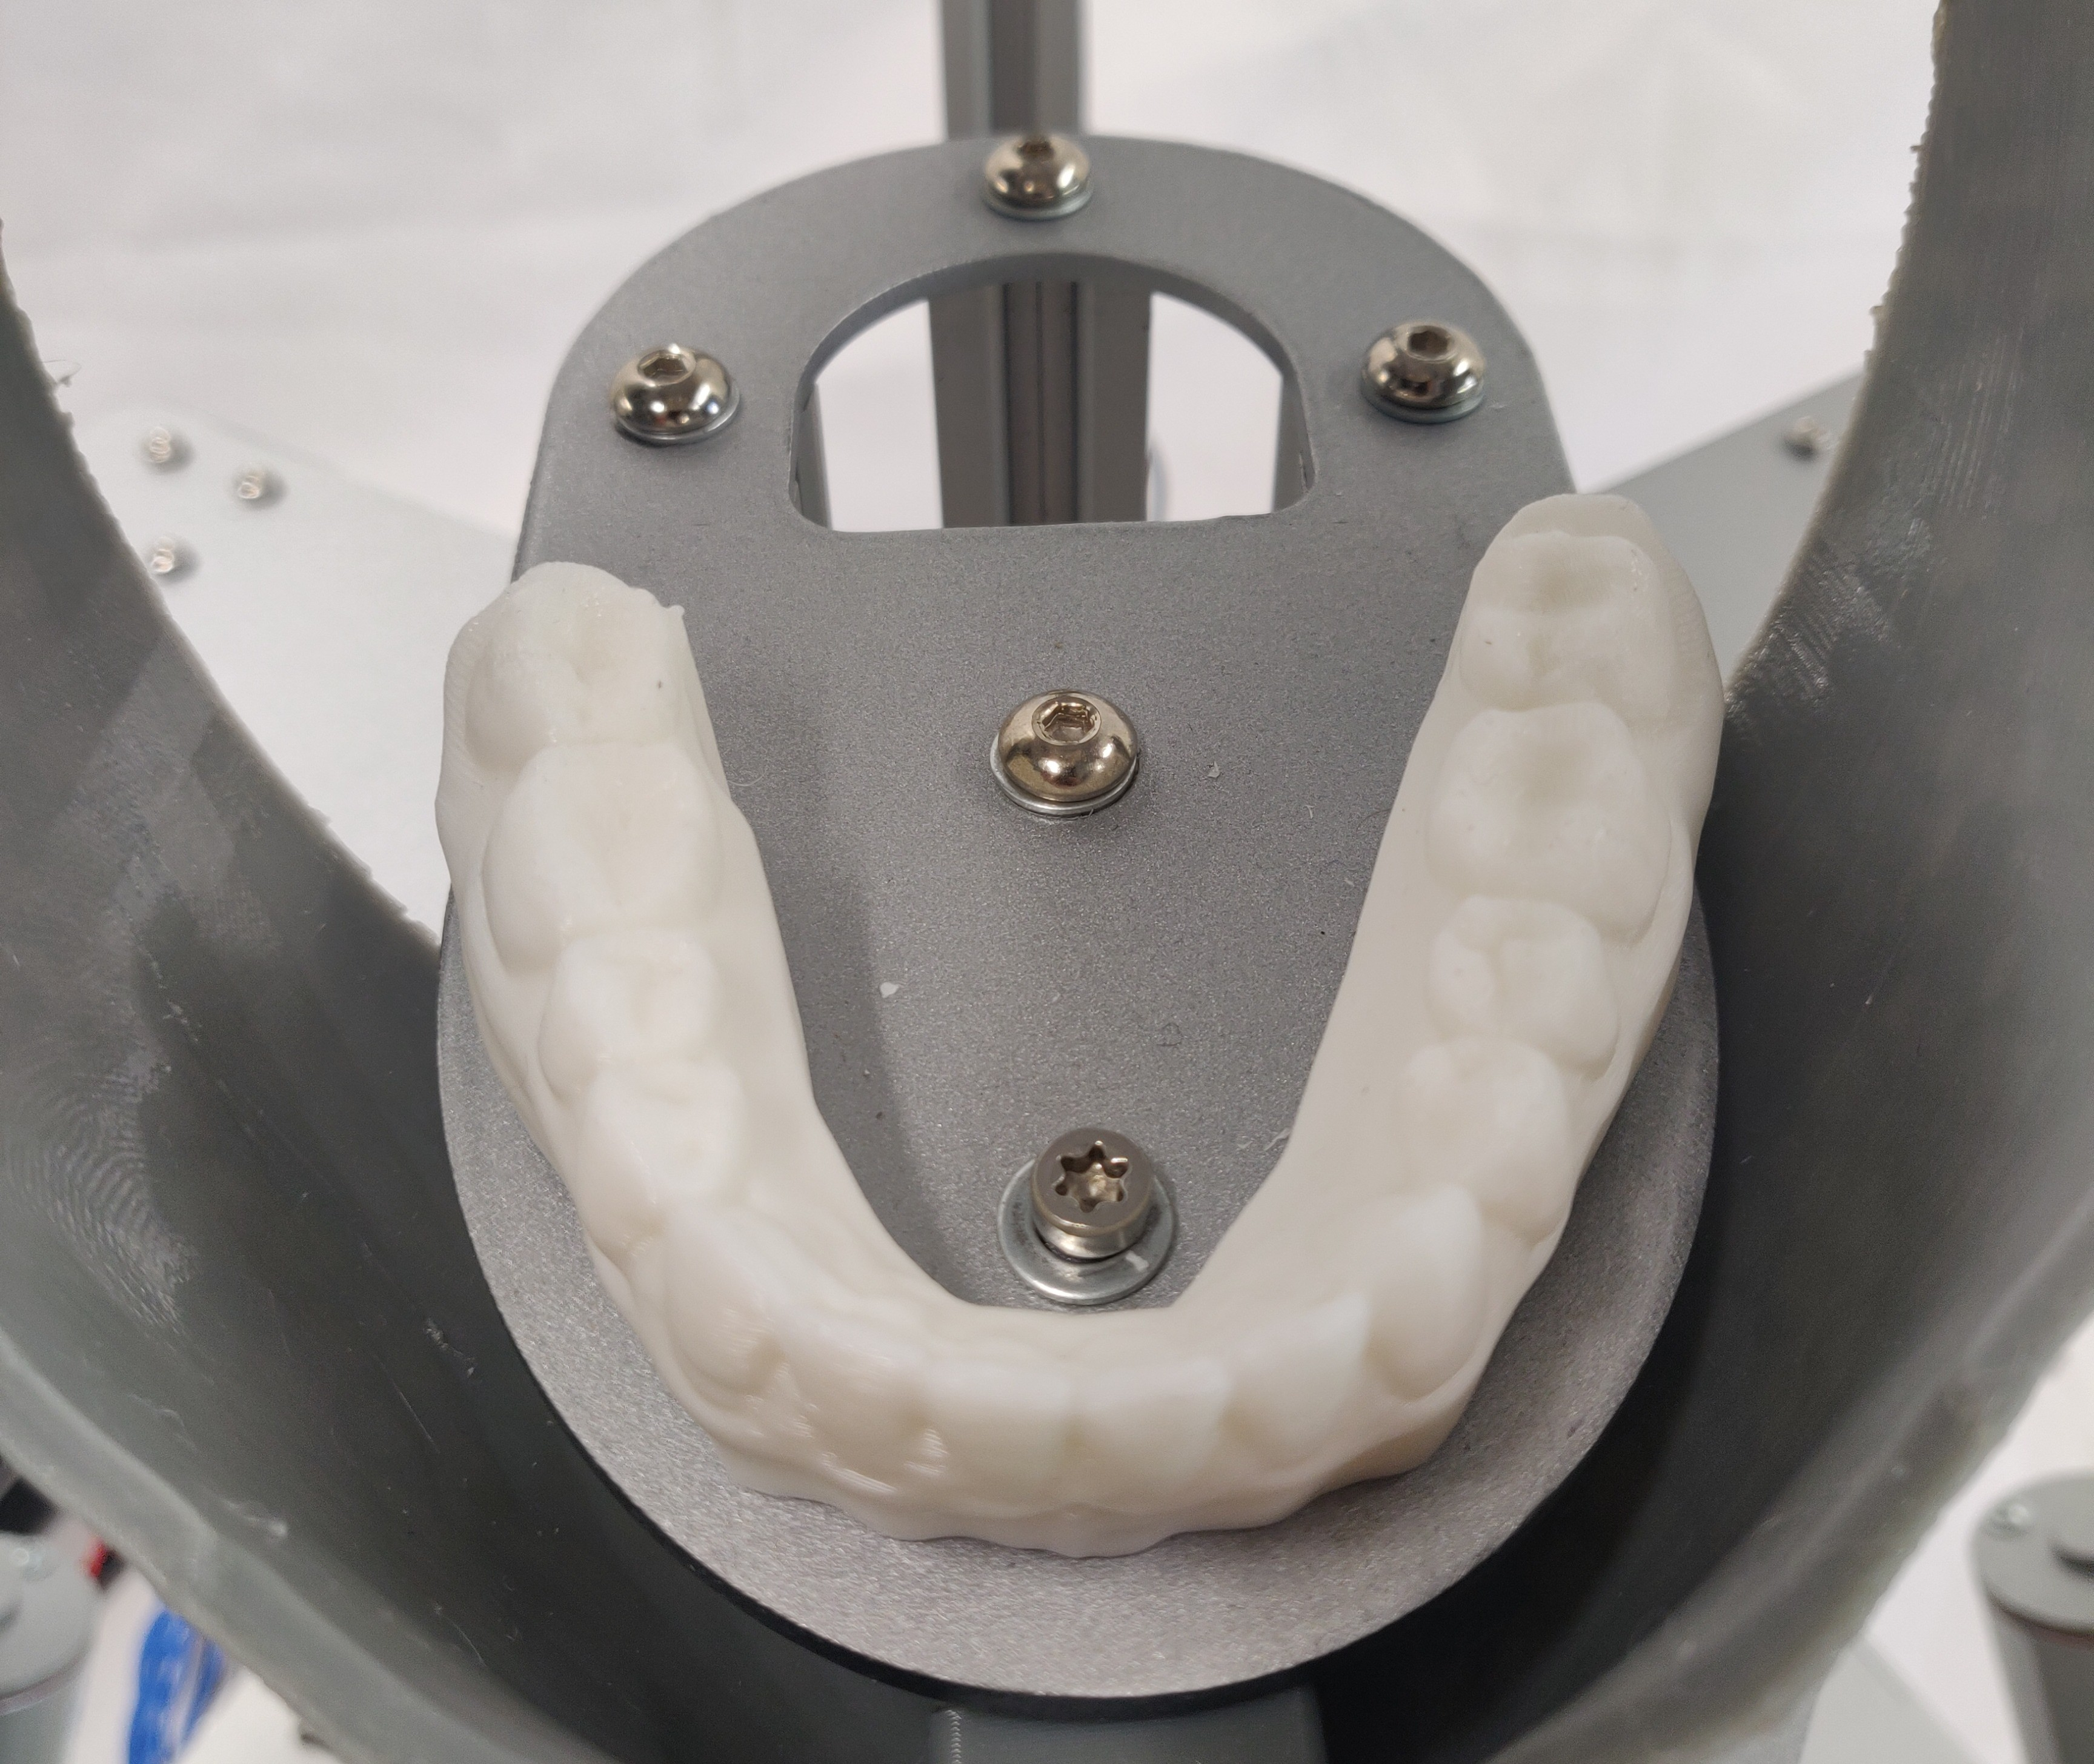
\includegraphics[width=0.6\textwidth]{figures/lower_jaw_close_up.jpg}
    \caption{Picture of the lower jaw close-up.}
    \label{fig:pic_lower_jaw_close_up}
\end{figure}

\begin{figure}[H]
    \centering
    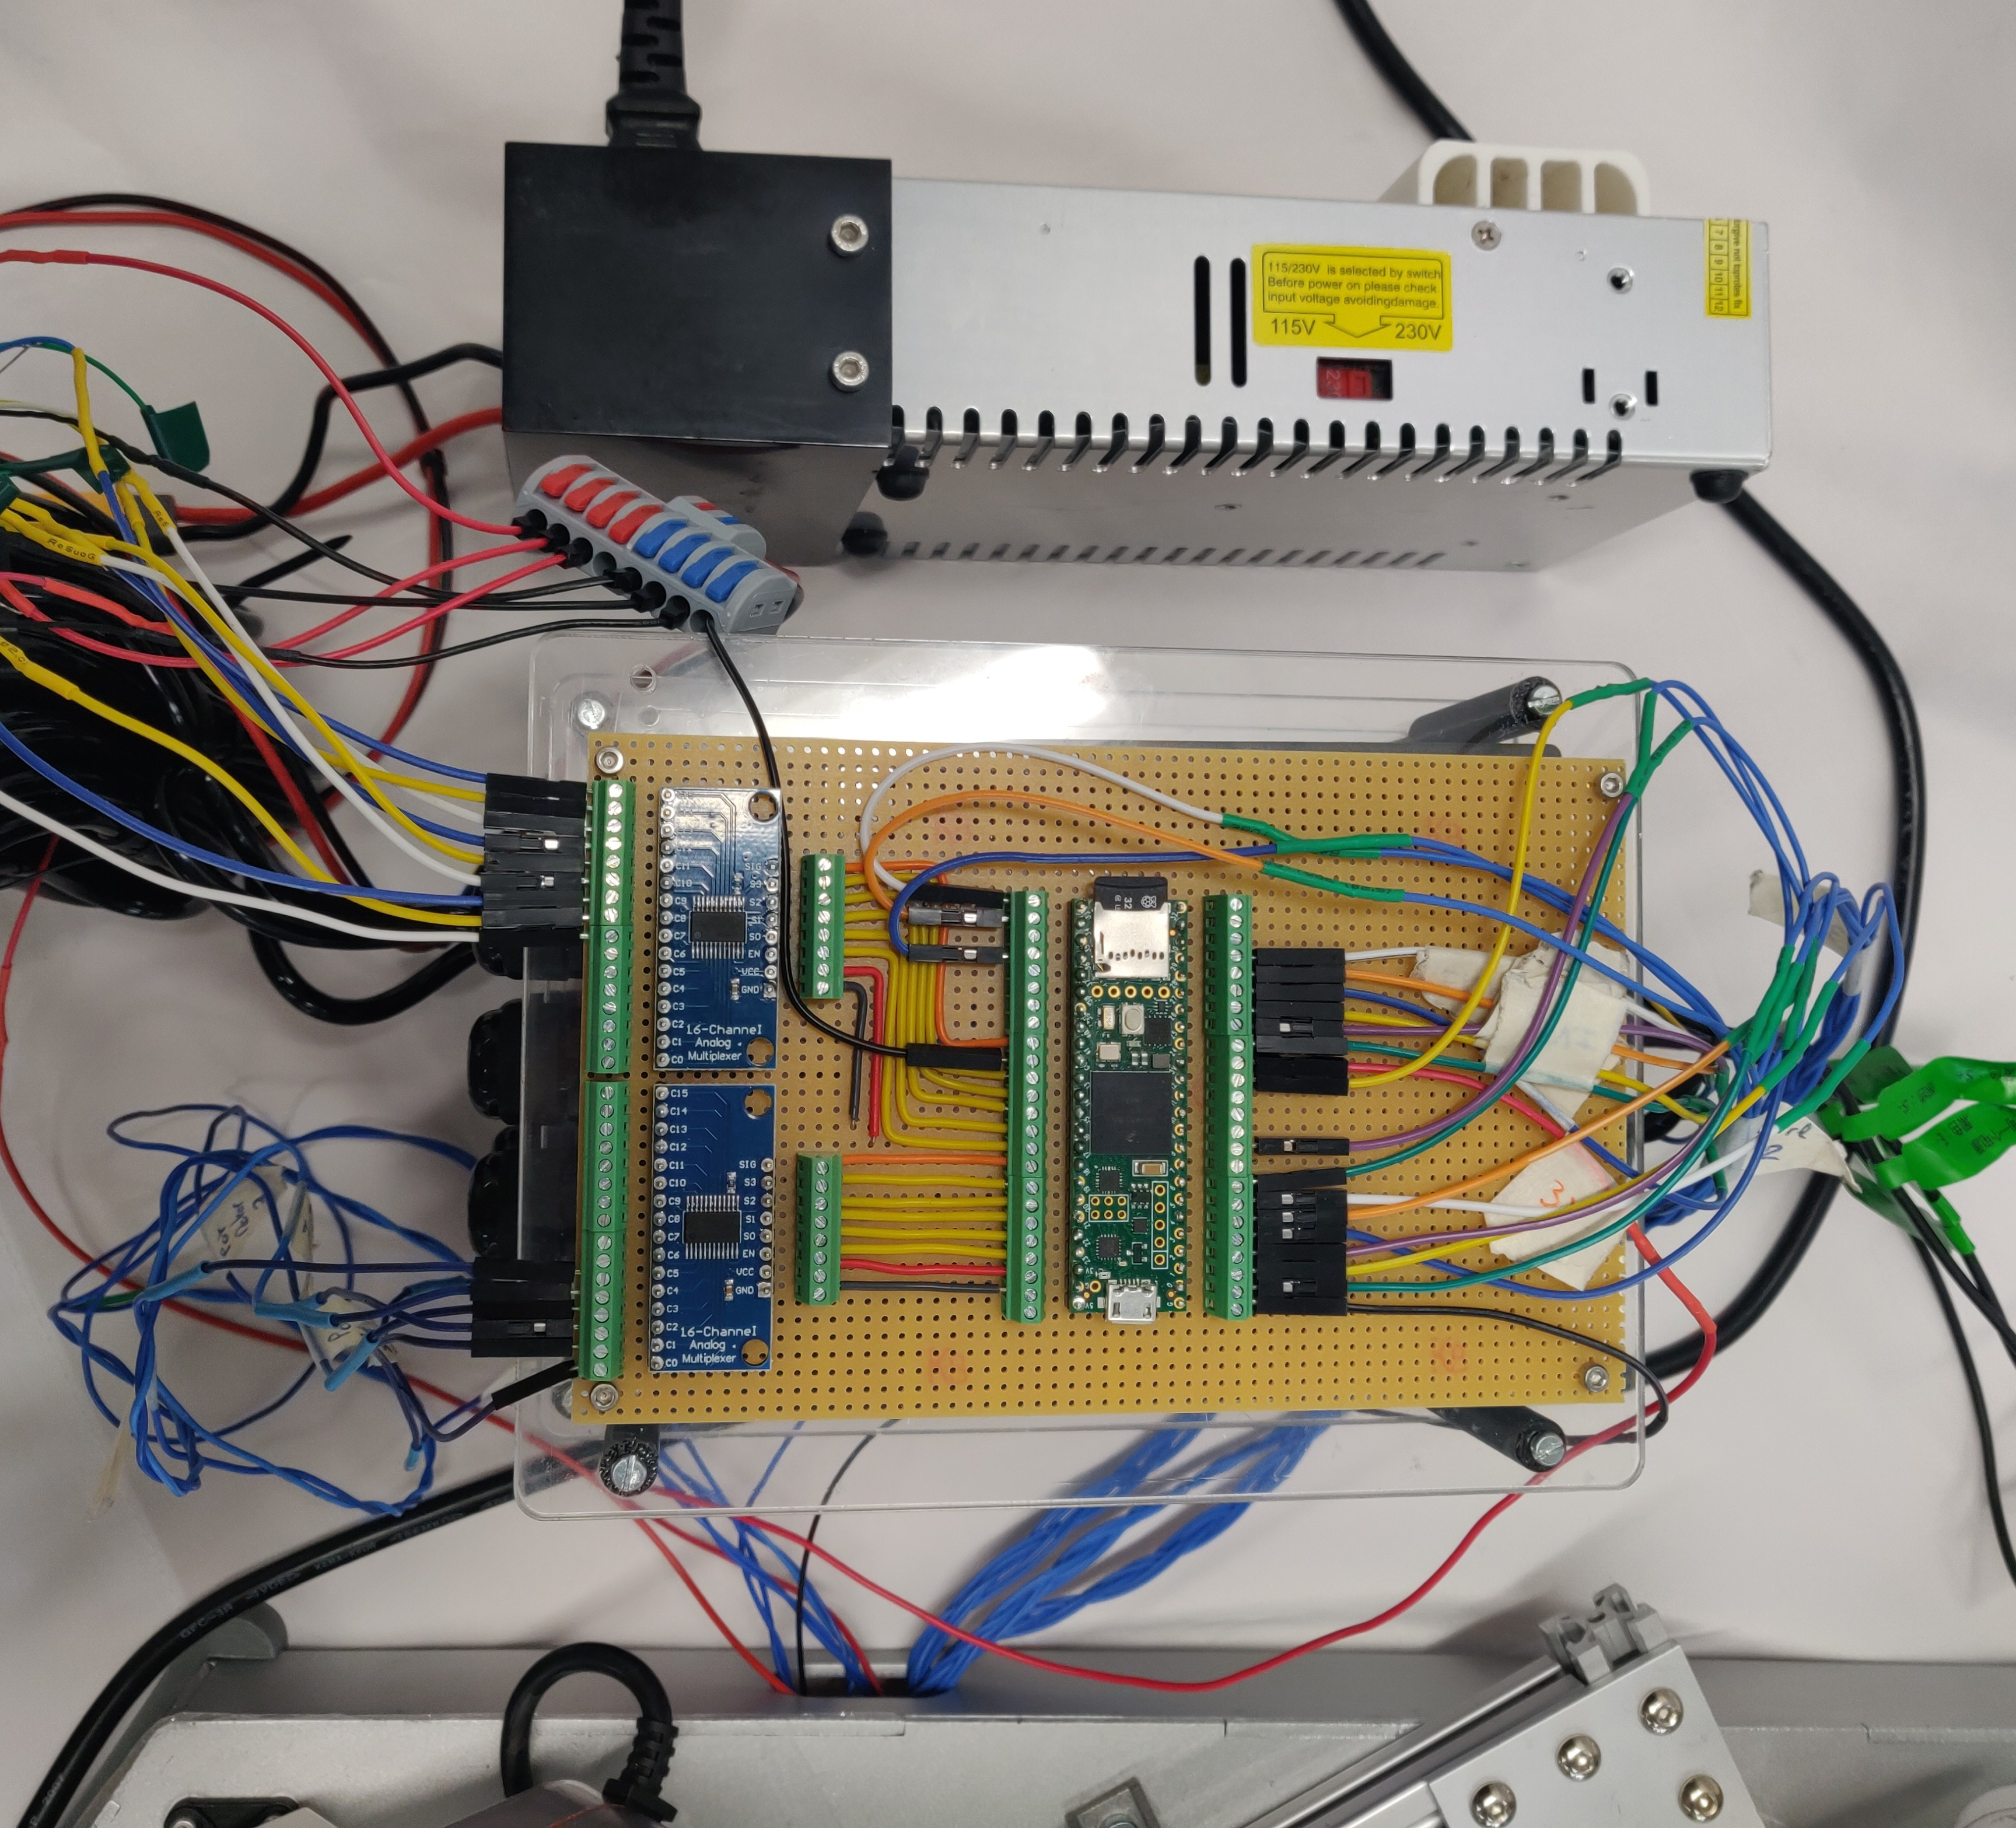
\includegraphics[width=0.7\textwidth]{figures/elec_close_up.jpg}
    \caption{Picture of the main electronics close-up.}
    \label{fig:pic_elec_close_up}
\end{figure}

\subsection{Electronics connections to Teensy~4.1}

\begin{figure}[H]
    \centering
    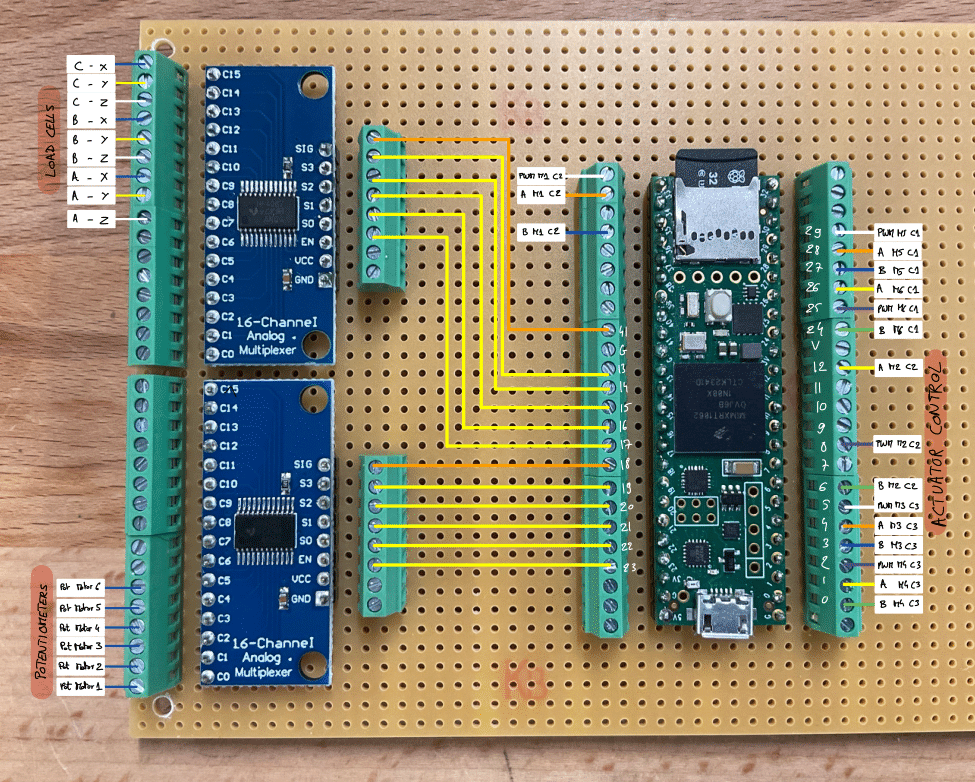
\includegraphics[width=\textwidth]{figures/elec_connections.png}
    \caption{Connections to Teensy~4.1. \textit{Notes: } "PWM M1 C2" refers to the PWM signal for motor 1 connected to controller number 2, 
    'A - X' refers to analog input for load cell A (front) axis X, "Pot Motor 1" refers to the potentiometer for motor 1.}
    \label{fig:connections_teensy}
\end{figure}

\begin{table}[h]
    \centering
    \begin{tabular}{|c|c|c|}
        \hline
        \textbf{Motor} & \textbf{Controller} & \textbf{Output} \\ \hline
        Motor 1 & \multirow{2}{*}{Controller 2} & Motor1 output \\ \cline{1-1} \cline{3-3}
        Motor 2 &  & Motor2 output \\ \hline
        Motor 3 & \multirow{2}{*}{Controller 3} & Motor1 output \\ \cline{1-1} \cline{3-3}
        Motor 4 &  & Motor2 output \\ \hline
        Motor 5 & \multirow{2}{*}{Controller 1} & Motor1 output \\ \cline{1-1} \cline{3-3}
        Motor 6 &  & Motor2 output \\ \hline
    \end{tabular}
    \caption{Motor-to-controller output connections.}
\end{table}